\documentclass[bottom=1in, 10pt]{LatexClass/ulthesis}


\usepackage{epsfig}
\usepackage{amssymb}
\usepackage{amsmath}
\usepackage{amsfonts}
\usepackage{graphicx}
\usepackage{amsthm}
\usepackage{algorithm}
\usepackage{algorithmic}
\usepackage{fancybox}
%\usepackage{subfigure}
\usepackage{multirow}
\usepackage{cite}
\usepackage{perpage} %the perpage package
\usepackage{subcaption}
\usepackage{caption}
\usepackage{slashbox}
\MakePerPage{footnote} %the perpage package command
\newtheorem{mydef}{Definition}

% For not placing figures on pages by themselves and wasting space.
\renewcommand{\topfraction}{0.85}
\renewcommand{\textfraction}{0.1}
\renewcommand{\floatpagefraction}{0.75}
\renewcommand{\listalgorithmname}{LIST OF ALGORITHMS}

\centerchapter

\doublespace

\phdthesis

\begin{document}

\renewcommand{\thesisauthor}{Ameni Trabelsi}
\renewcommand{\thesismonth}{May}
\renewcommand{\thesisyear}{2018}
\renewcommand{\thesisabstractdate}{April $24^{th}$, 2018}
\renewcommand{\thesistitle}{\normalfont{MACHINE LEARNING FOR OMICS DATA ANALYSIS}}
\renewcommand{\thesistype}{A Thesis Submitted to the Faculty of the J.B. Speed School of Engineering of the University of Louisville in Partial Fulfillment of the Requirements}
\renewcommand{\thesisdegree}{Master of Science}
\renewcommand{\thesisdegreeabbreviation}{M.S.}
 \renewcommand{\thesiscommitteesize}{2}
\renewcommand{\thesisauthorpreviousdegrees}
{B.E., Tunisia Polytechnic School, 2016}
\renewcommand{\thesisauthoraddress}{Department of Computer Engineering and Computer Science \\
   University of Louisville, \\Louisville, KY}



%% For proposal
\proposaltitlepage                   %% Generate the proposal title page.
\thesiscopyright
\clearpage\mbox{}
\thispagestyle{empty}
\addtocounter{page}{-1}
\clearpage
\thesissignaturepage    
%% Following lines not needed for proposal
%%\thesistitlepage                     %% Generate the dissertation title page.
%%\thesissignaturepage                 %% Generate the signature page.

%%
%% This adds a "Page" subheading to the Table of Contents.
%% Do not remove this line.
%%




%\begin{thesisacknowledgments}
\indent I would like to convey my special regards to my distinctive advisor, Dr. Hichem Frigui who supported my work in this way and helped me get results of better quality and overcome numerous obstacles. \\ 
\indent My sincere thanks also goes to Dr. Xiang Zhang. His guidance helped me in all the time of research and steered me in the right direction whenever he thought I needed it. \\
\indent I also thank  Dr. Juw Won Park for accepting to serve in my thesis committee and being a part of this special milestone.\\
\indent I address, likewise, my thanks to my colleagues in the Multimedia Research Laboratory, and the Computer Engineering and Computer Science Department for their support and friendship. \\ 
\indent Finally, I want to convey my very profound gratitude to my family for their continuous support and unconditional love throughout my years of study and through the process of researching and writing this thesis.
\begin{thesisabstract}
In proteomics and metabolomics, to quantify the changes of abundance levels of biomolecules in a biological system, multiple sample analysis steps are involved. The steps include mass spectrum deconvolution and peak list alignment. Each analysis step introduces a certain degree of technical variation in the abundance levels (i.e. peak areas) of those molecules. Some analysis steps introduce technical variations that affect the peak areas of all molecules equally while others affect the peak areas of a subset of molecules with varying degrees. To correct these technical variations, some existing normalization methods simply scale the peak areas of all molecules detected in one sample using a single normalization factor or fit a regression model based on different assumptions. As a result, the local technical variations are ignored and may even be amplified in some cases.\\
\indent To overcome the above limitations, we developed a molecule specific normalization algorithm, called MSN, which adopts a robust surface fitting strategy to minimize the molecular profile difference of a group of house-keeping molecules across samples. The house-keeping molecules are those molecules whose abundance levels were not affected by the biological treatment. We also developed an outlier detection algorithm based on Fisher Criterion to detect and remove noisy data points from the experimental data. The applications of the MSN method on two different datasets showed that MSN is a highly efficient normalization algorithm that yields the highest sensitivity and accuracy compared to five existing normalization algorithms. The outlier detection algorithm's application on the same datasets has also shown to be efficient and robust.
\end{thesisabstract}

\tableofcontents

\listoftables

\listoffigures

%\listofalgorithms
%\addcontentsline{toc}{part}{LIST OF ALGORITHMS}

\addtocontents{toc}{\protect \contentsline {part} {} {}}
\addtocontents{toc}{\protect \contentsline {part} {CHAPTER} {Page}}

\addtocontents{lof}{\protect \contentsline {part} {FIGURE} {Page}}
\addtocontents{lot}{\protect \contentsline {part} {TABLE} {Page}}
\addtocontents{loa}{\protect \contentsline {part} {ALGORITHM}{Page}}

\renewcommand{\thefigure}{\thechapter.\arabic{figure}}
\renewcommand{\thetable}{\thechapter.\arabic{table}}
\renewcommand{\thealgorithm}{\thechapter.\arabic{algorithm}}
\renewcommand\theequation{\thechapter.\arabic{equation}}
\numberwithin{algorithm}{chapter}
\numberwithin{equation}{chapter}
\numberwithin{figure}{chapter}
\numberwithin{table}{chapter}

%% Start each new "Chapter" with the "\chapter{}" command
%% Use "\label{}" to mark the chapter so that
%% you may later refer to it with a line such as
%% "... as discussed in Chapter~\ref{chap:intro} ..."

\chapter{INTRODUCTION}
Proteomics and metabolomics are the studies of proteomes and metabolomes, respectively. To discover biomarkers that caused the differences between control samples and treatment samples and to reveal the metabolic and proteomic changes caused by a biological event, multiple biological replicates are used in each sample group to increase the statistical power of biological interpretation of omics data.\\
\indent Efficient and robust tools are needed to perform accurate and precise quantification to examine the true concentration differences of individual molecule found in different samples involved in the omic analysis. These include biological work (e.g., sample collection), analytical work
(e.g., sample analysis) and data analysis (e.g., feature extraction, outlier detection and quantification). Various procedures at each analysis step can influence the quantitative results significantly and thus should be performed with great care. In addition to the technical variations, proteomics and metabolomics data also include biological variations. The goal of data analysis in these applications is to reduce the technical variations while preserving the biological variations. 

\section{Liquid Chromatography Mass Spectrometry LC-MS data}
\indent Liquid chromatography (LC) is a strategy that separate biomolecules using two immiscible phases, i.e., stationary and mobile \cite{lcms}.\\
 Mass spectrometry (MS) is an analytical technique that measures the mass-to-charge (m/z) ratio of charged particles (ions)\cite{lcms}. Despite the fact that there is a wide range of different types of mass spectrometers, all of them make use of electric or magnetic fields to control the movement of particles delivered from an analyte of interest and decide their m/z values. The basic components of a mass spectrometer are the ion source, the mass analyzer, the detector, and the data and vacuum systems.\\
\indent Coupling MS with LC is alluring in light of the fact that fluid chromatography can isolate molecules in complex natural mixtures by their interaction difference between mobile phase and stationary phase, while MS further separate them by m/z values. These two separation methods are orthogonal. These days, LC-MS has turned out to be a standout amongst the most broadly utilized chemical analysis techniques \cite{lcms2}.\\
\indent Advantages of the LC-MS include high sensitivity and the ability to discriminate between thousands of features in a single experiment. But like any high-throughput technology, there are always systematic biases in omics data acquired by LC-MS. As we increase the number of samples in the dataset, we also boost the possibility of a time dependent variation in the resulting molecule data. The trends in time in LC-MS data are usually due to drifts in analyte retention time caused by changes in the performance of the LC column or due to variations in signal intensity caused by fluctuations in MS sensitivity. These issues could be avoided partly by careful experimental design or by using quality control samples. However, there is always a need for robust data normalization. Flexibility is a very important criteria for normalization methods since biases can be of arbitrary complexity and also overfitting should be avoided.

\section{Analysis of Liquid Chromatography Mass Spectrometry Data}
Several software packages have been developed to analyze LC-MS data \cite{lcms2}. The analysis include several components as summarized in Figure \ref{flo}. The first component, Spectrum Deconvolution, consists of reducing the data acquired from the experiments into a peak list. It involves baseline correction, denoising, peak detection, resolving overlapping peaks, etc \cite{specdeco}.\\
\indent Mass spectrum centralization is the first step in Spectrum Deconvolution. Two main options are used to centralize the mass spectra acquired under profile mode: second-order polynomial fitting based
local maxima (SPF-LM) and one-dimensional discrete
wavelet-transform (1-DWT). The SPF-LM consists in applying a first-derivative operation to first detect local maxima in the spectrum. Then, it applies a second-order polynomial fitting (SPF) to fit the local peaks. This step serves to identify the m/z values of the detected peaks and their intensities. In the 1-DWT, we first apply a one-dimensional discrete wavelettransform to each mass spectrum, then we detect local maxima in the wavelet domain to determine the m/z values of the peaks and their intensities.\\

Next, the selected ion chromatogram
(XIC) is usually constructed by selecting all signals that have an
m/z value matched to the m/z value of an ion of interest, with a
user defined variation window.
\begin{figure}
	\centering
	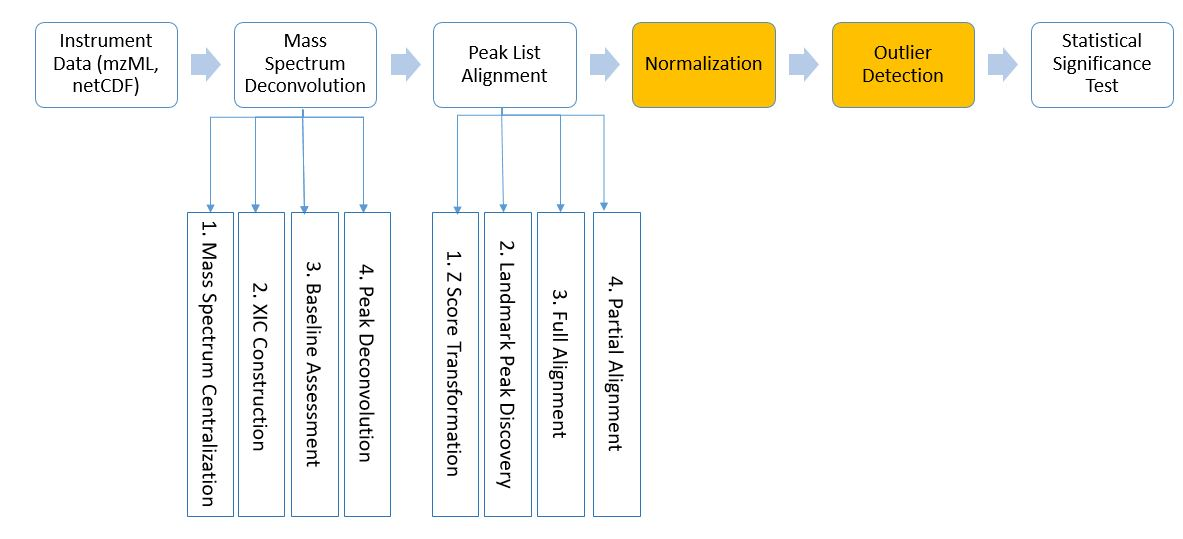
\includegraphics[width=16cm]{flow_data_process.JPG}
	\caption{Flowchart of LC-MS data analysis.}
	\label{flo}
\end{figure}

To calculate the area of a chromatographic peak from an XIC \cite{xic}, two approaches are usually used. The first approach sums all signals belonging to the chromatographic peak, while the other approach fits the chromatographic peak with a predefined peak model.\\
\indent The next component in the LC-MS data analysis is the peak list alignment \cite{lcms2}. The first step consists in applying z-score transformation to the retention time values to transform them into a normal distribution. This step is necessary to make the alignment of heterogenous experimental data possible mainly because experimental data is acquired under various experimental conditions.

For the actual alignment step, a peak list is selected as a reference and the rest of the
peak lists are aligned with respect to this reference. There are two steps of alignment; the full alignment followed by the partial alignment. The main purpose of full alignment is to identify
the landmark peaks, these are the set of metabolite peaks
generated by the same type of metabolites present in
every sample. In the partial alignment step, the peaks in a test sample
that are not recognized as the landmark peaks are aligned.\\
\indent To summarize, several analysis steps are involved in detecting molecular peaks from massive LC-MS data. Noise can be introduced at any of these steps. This noise is cumulated with the experimental errors to give highly noisy data. Thus, the next two components of LC-MS data analysis consist of data normalization and outlier detection. These two steps are required before analyzing the data and extracting information. 
Finally, an abundance test, such as the pairwise two-tail t-test, is performed on the normalized and cleaned peak areas to detect
the abundance changes of each metabolite between two sample
groups.

\section{Research Motivations} 
In proteomics and metabolomics, some analysis steps introduce technical variations that affect the peak areas of all molecules equally while others affect the peak areas of a subset of molecules with varying degrees. For instance, the inherent variability in the position of the syringe plunger position occurs whenever it is moved by the autosampler, which can easily introduce 2 \% variation in volume for all molecules (i.e. global technical variations). However, some data analysis algorithms have poor performance in deconvoluting overlapping chromatographic peaks, resulting in large variations in the peak areas of low abundance molecules (i.e. local technical variations). To correct these technical variations, existing normalization methods can only address the global technical variations. As a result, the local technical variations are ignored and may even be amplified in some cases.\\
While different normalization methods have been developed, these methods normalize the
abundances of all molecules detected in a sample based on certain assumptions \cite{clevland}\cite{astrand:eke}. However, these assumptions  usually do not hold for biological systems and may introduce biases in the normalized data.\\



The discovery of observations that deviates from normal behavior also known as outlier detection has
been widely studied in recent years \cite{outlier} \cite{outlier2}, resulting in a set of algorithms designed
to detect these rare but potentially crucial events. In some specific contexts an
outlier is a data point that can be considered either as an abnormality or noise.
The effect of undetected outliers in different application domains can have serious and disastrous
consequences. An example is the detection of landmines where an undetected
positive case implies an undetected landmine; another example is a failed attempt to
detect strange behavior in the use of a stolen credit card resulting in a financial
impact for the credit card holder. In both of these examples, the minority of the
cases represents the class of interest.

\section{Contributions}
 In this thesis, we focus on the two major steps highlighted in Figure \ref{flo} which are the normalization and outlier detection steps.
For outlier detection, the goal is to eliminate noisy undesired peaks.
We propose an algorithm that is based on the Fisher Criterion to detect the data points that lead to a remarkable change (whether increase or decrease) in the proposed criteria. The performance and robustness of the proposed method is validated using several experiments with real data sets.\\
\indent For the second contribution, we propose a molecule specific normalization algorithm, called MSN. MSN first identifies potential house-keepings, a group of molecules whose abundance levels were not affected by the biological treatment. MSN then adopts a robust surface fitting strategy to minimize the molecular profile difference of the house-keeping molecules across samples. Using different data sets, we compare our proposed MSN to several state-of-the-art normalization methods used for this application.

\indent The organization of the rest of this thesis is as follows. Chapter 2 provides a review of existing methods of normalization and outlier detection of omics data.
In chapter 3,  we  introduce our Fisher criterion based outlier detection and our molecule specific normalization and describe the different steps involved. In chapter 4, we describe the evaluation results of the proposed methods using our LC-MS metabolomics data set that motivated our approach, as well as the evaluation results using a publically available LC-MS proteomics data set. Then, we report the results of our experimental evaluations. Finally, we provide our concluding remarks and potential future work in chapter 5.

\chapter{LITERATURE REVIEW}
The analysis of LC-MS data involves several steps as explained in the previous chapter and summarized in Figure \ref{flo}. In this chapter, we review related work in the last two components that are relevant to our proposed methods, namely, outlier detection and normalization.
\section{Notations}

For the rest of this thesis, we assume that the input data $P$ is available in an $ M \times N$ matrix form, i.e., $P=[P_{ki}]$ for $ k=1\dots M$ and $i=1 \dots N$, where $M$ is the number of features and $N$ is the number of samples. We also assume that the samples belong to two groups: $g=0,1$, with $n_g$ samples per group, i.e., $n_0+n_1=N$. Normalization methods that are described below have been proposed for cDNA arrays or metabolomic applications. In cDNA array, $P_{ki}$ refers to probe intensity of probe k in array i. While in metabolomic data, $P_{ki}$ refers to peak area of compound k in sample i. For both applications when data involve more than two groups, typically, they will be treated two groups at a time.



\section{Outlier Detection Methods}

\subsection{ Statistical Methods}
\subsubsection{Boxplots for outlier detection}

\indent Box plots \cite{tukey} are non-parametric outlier detection methods. They analyze the variation in samples of a statistical population without making any assumptions about the underlying statistical distribution.  The interquartile range (IQR) is calculated by the difference between the two quartiles Q1 and Q3, i.e. $IQR = Q3 - Q1 $


\begin{figure}
	\centering
	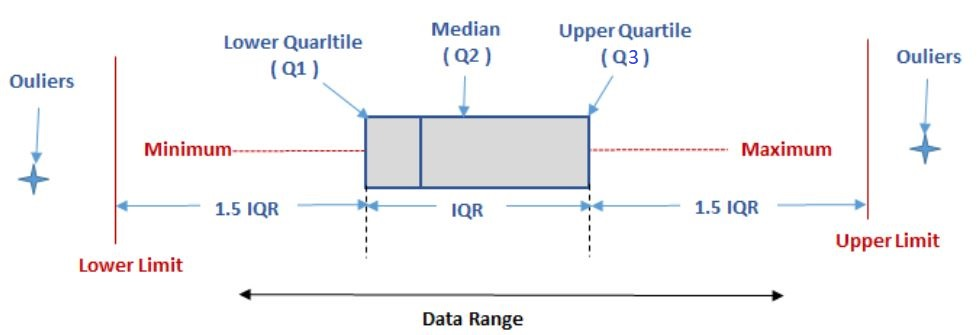
\includegraphics[width=15cm]{boxplot}
	\caption{Box Plot Diagram to identify outliers }
	\label{box}
\end{figure}


The quartiles, Q1 and Q3, are calculated such that the integral of the PDF from $-\infty$ to Q1 equals 0.25 and that of Q3 to $+ \infty$ is 0.75.
Figure \ref{box} depicts a diagram of box plots to detect outliers. In this figure, the factor K is set to 1.5. A point is considered as an outlier if it is not in the range of [Q1 – 1.5 x IQR , Q3 + 1.5 x IQR].\\

\subsubsection{GRUBBS}

Grubbs \cite{grubbs}\cite{stefansky} is an outlier detection algorithm that assumes normality of the distribution. This test detects at most one outlier at a time. It is applied repeatedly until no outliers can be detected. The data is first sorted and then Grubbs tests if the maximum $P_{\max }$ or the minimum $P_{\min }$ data point is an outlier.\\ First, it computes G using:\\
\begin{eqnarray}\label{eq:grubbs}
G_{min}={\frac  {{\bar  {P}}-P_{\min }}{s}} , \text{ and   }
G_{max}={\frac  {P_{\max }-{\bar  {P}}}{s}}
\end{eqnarray}
In Equations (\ref{eq:grubbs}), $\bar{P}$ is the mean of the data points, and $s$ is the standard deviation  computed using:
\begin{eqnarray}\label{std}
s= \sqrt{\frac{1}{N-1}\sum_{i=1}^{N}(P_i-\bar{P})^2}
\end{eqnarray} 
Then, for the two sided test, it compares $G_{min}$  to the threshold using:
\begin{eqnarray}\label{eq:testg}
 G_{min}>{\frac  {N-1}{{\sqrt  {N}}}}{\sqrt  {{\frac  {t_{{\alpha /(2N),N-2}}^{2}}{N-2+t_{{\alpha /(2N),N-2}}^{2}}}}} 
\end{eqnarray}
In (\ref{eq:testg}), $N$ is the number of samples, and $t_{\alpha/(2N),N - 2}$ denotes the upper critical value of the t-distribution with $N - 2$ degrees of freedom and a significance level of $\alpha/(2N)$. If the condition in (\ref{eq:testg}) is satisfied, then $P_{min}$ is identified as an outlier.
Similarily, $G_{max}$, is compared to the threshold in (\ref{eq:testg}) to check if $P_{max}$ is an outlier.
If the one-sided test is used, in equation (\ref{eq:testg}), we replace $\alpha/(2N)$ with $\alpha/N$.
\\
If neither $G_{max}$ nor $G_{min}$ satisfy the in equation (\ref{eq:testg})  are passed, both the min and max are tested for being outliers. First, we compute G using:
\begin{eqnarray}\label{eq:geq}
G={\frac  {P_{\max }-P_{\min }}{s}}.
\end{eqnarray}
Then, we compare G to a threshold and check if:
\begin{eqnarray}\label{eq:geqq}
 G>{\sqrt  {{\frac  {2(N-1)t_{{\alpha /(N(N-1),N-2)}}^{2}}{N-2+t_{{\alpha /(N(N-1),N-2)}}^{2}}}}} 
\end{eqnarray}
In equation (\ref{eq:geqq}), $t_{(\alpha/N(N-1),N-2)} $ denotes the $\alpha/N(N-1)$ percentile of the t-distribution with (N-2) degrees of freedom. If the condition in equation (\ref{eq:geqq}) is satisfied, then both the minimum and the maximum are outliers.\\
\subsubsection{Generalized Extreme Studentized Deviate (GESD)}
GESD \cite{Rosner} is similar to Grubbs and it requires a prior knowledge of the maximum number of outliers to be removed $r$.
To compute GESD, we first compute $R$ , using: 
\begin{eqnarray}
R=\max_{i=1..N}{\frac{|P_i-\bar{P}|}{s}}.
\end{eqnarray}
Then, we remove the data point $P_i$.
Similarly, we compute $R_2$ for the remaining observations (after deleting $P_i$) and delete the $P_j$ that maximizes $R_2$. After repeating the above step $r$ times and computing $R_1, R_2 \dots R_r$, we compare each $R_i$ with $\lambda_i$ and remove the data point that corresponds to the $R_i$ such that $R_i > \lambda_i$ where $\lambda_i$ is computed using:
\begin{eqnarray}
\lambda_i=\frac{t_{(p,N-i-1)}(N-i)}{\sqrt{(N-i-1+t_{(p,N-i-1)}^{2})(N-i-1)}}, \text{ $i=1,...,r$ and, } p=1- \frac{\frac{\alpha}{2}}{N-i+1}
\end{eqnarray}
\subsubsection{Z Score}
Z score \cite{boris} is similar to Grubbs and it assumes normality. First, we compute the zscore of each sample $P_i$ using:
\begin{eqnarray}
Z_{score}(i)=\frac{P_i- \bar{P}}{s},
\end{eqnarray}
The scores are then compared to a constant threshold and the outliers are defined as the data points that have a score larger than the threshold.



\subsubsection{Kimber GESD}
The kimber GESD \cite{kimber} \cite{kimber2} assumes Gamma distribution. It removes the largest observations from the upper end of the sample, starting
with the largest $r$ where $r$ is an input parameters.\\
 for $j = 1, 2, ... , r$ Kimber defines the test statistic $S_j$ by:\\
\begin{eqnarray}
S_j=\frac{P_{N+1-j}}{\sum_{i=1}^{N+1-j}P_i}, \text{ for $j= 1, \dots , r$}
\end{eqnarray}
Then, for $j = r, r- 1, ... , 1$, we check if $ S_j > s_j $, where $s_j=f(j,r,\alpha,N )$ is the appropriate critical value available in Kimber (Figure \ref{kimber}). The largest value of j, say $r*$, for which $S_{r*} > S_{r*}$ declares the upper $r*$ observations as outliers.

\begin{figure}\label{kimber}
	\centering
	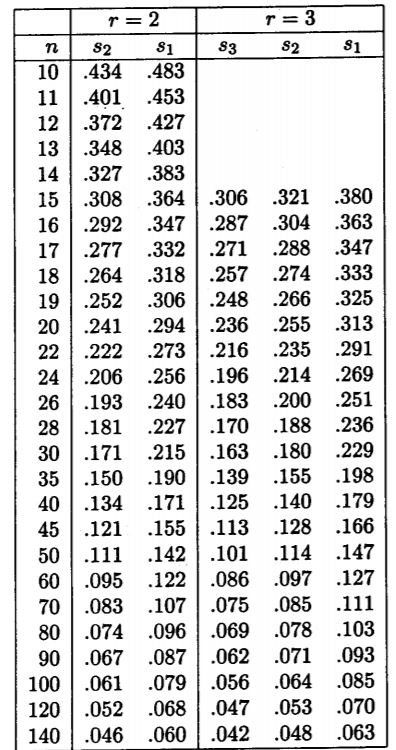
\includegraphics[width=8cm]{kimber}
	\caption{5 \% critical values for Kimber's test for finding up to r upper outliers from
		an exponential distribution }
	
\end{figure}

Table ~\ref{dico} is a summary of the different outlier detection algorithms along with the different  distributions they could be applied to. As it can be seen, Grubbs, GESD and Zscore can be applied to normal and lognormal distributions. On the other hand, Kimber can only be applied to Gamma distributions. Boxplots are the most general and can be applied to any statistical distribution.\\

\begin{table}[h!]
	\centering
	\caption{Applicability of various statistical outlier detection methods to data with the different distribuions}
	\begin{tabular}{|c|c|c|c|c|c |p{3cm}|} 
		\hline
		\textbf{Distribution} & \textbf{GRUBBS} & 	\textbf{GESD} &	\textbf{Kimber} & \textbf{Z Score} &	\textbf{Box Plot}  \\ [0.5ex] 
		\hline\hline
		\textbf{Normal} & x &x& &x&x \\
		\hline
		\textbf{Lognormal} & x &x& &x&x  \\
		\hline
		\textbf{Binomial} & & & & & x  \\
		\hline
		\textbf{Geometric} & & & & & x  \\ 
		\hline
		\textbf{Poisson} & & & & & x  \\
		\hline
		\textbf{Gamma} & & &x & & x  \\
		\hline
	\end{tabular}
	\label{dico}
\end{table}

\subsection{Minimum Volume Ellipsoid}
The Minimum Volume Ellipsoid (MVE) is a common approach used for robust outlier detection in multivariate space  \cite{mve}. It takes subsamples of the dataset and calculates the volume of the ellipsoid that encloses the subsample. The main idea is that outliers increase the volume of the ellipsoid dramatically. Thus, the MVE will correspond to the actual core of the dataset after eliminating outliers. We can consider the samples as ordered by the probability of being an outlier. The first sample is the least probable to be an outlier and the last is the most probable to be an outlier.\\
\indent In the following, we illustrate the MVE with a simple example that includes 10 2-D data points. In figure ~\ref{mve}, different ellipsoids are drawn each time after deleting one outlier at a time. As it can be seen the volume of the ellipsoid has decreased remarkably after deleting the third outlier. In figure ~\ref{mve2}, we plot the evolution of the volume of the ellipsoid as a function of the number of samples each time one sample is identified as outlier and removed. We notice that there is a sudden increase after adding the 8th sample. This increase continues after adding the 9th and the 10th sample. We can conclude that most likely the 8th, 9th and 10th samples are outliers.\\



\begin{figure}
	\centering
	\begin{subfigure}[b]{0.5\textwidth}
		\centering
		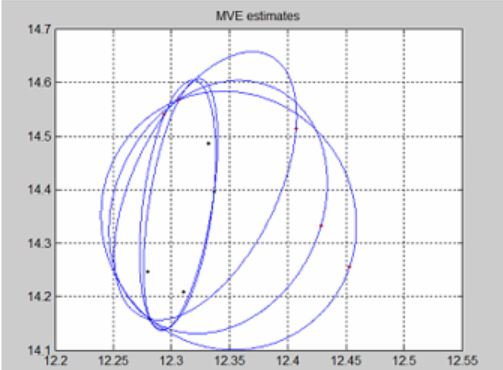
\includegraphics[height=1.9in]{MVEll.JPG}
		\caption{Example Ellipsoids contouring data points Each time after excluding one data point}
		\label{mve}
	\end{subfigure}%
	~ 
	\begin{subfigure}[b]{0.5\textwidth}
		\centering
		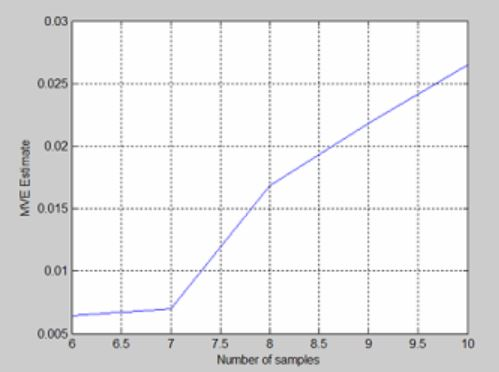
\includegraphics[height=1.9in]{MVEll2.JPG}
		\caption{MVE Estimate (y axis) and sample number (x axis)}
		\label{mve2}
	\end{subfigure}
	\caption{MVE example}
\end{figure}


At the core of the MVE algorithm is the identification of the outlier at each iteration or how to order the samples by their probability of being outliers.
At each iteration, one data sample is chosen as the most probable to be an outlier. We first calculate the Mahalanobis distance matrix of the data points using:
\begin{eqnarray}\label{eq:mve}
M= (X-E) Cov^{-1} (X-E)'
\end{eqnarray}

where $X$ is an ($n \times k$) matrix that include $k$ random features of the $n$ samples. Typically, we choose k=2. In equation (\ref{eq:mve}), $E$ is an $n \times 1$ vector where each component is the mean of the $k$ features, and $cov$ is the covariance matrix of the $n$ samples. Then, we determine the eigenvalues of M and choose the greatest eigenvalue. The data point that has the greatest eigenvalue is the most probable to be an outlier. These steps are repeated at each iteration after removing the identified outliers.

\section{Scaling Methods}
\indent Auto scaling is among the simplest and most common statistical normalization methods. It considers the z score of each data point instead of its initial value along each feature. This method works well when each attribute of the data follows a normal distribution. Since the standard deviation is used as the scaling factor, each normalized feature will have a unit standard deviation and therefore the data can be analyzed on the basis of correlations instead of covariances. Another variation of this method is the Pareto Scaling, where the scaling factor is the square root of the standard deviation \cite{berg:tar}: 
\begin{eqnarray}
P'_{ij}= \frac{P_{ij} - \mu_j}{\sqrt{s_j}}
\end{eqnarray}
Variable Stability Scaling \cite{berg:tar} is another extension of auto-scaling. It uses the coefficient of variation (cv) as a scaling factor. The  cv is defined as the ratio of the standard deviation to the mean, i.e., $ \frac{s}{\mu}$. Using this method, more importance will be attributed to the features that are more stable, i.e. having smaller variation.\\
\indent Range scaling, also known as feature scaling or min-max scaling, is another method that uses the range of the data as a normalization factor. Typically, the range is computed as the difference between the minimal and the maximal value of each feature:
\begin{eqnarray}
P'_{ij}= \frac{P_{ij} - \min_i{P_ij}}{\max_{i}{P_ij}- \min_{i}{P_ij}}
\end{eqnarray}
\section{Data Normalization Methods }
Normalization methods are not restricted to scaling. In fact, several other approaches have been introduced to reduce data variations. These include transformation methods like log transformation, which is usually used to convert multiplicative relations into additive ones to correct heteroscedasticity \cite{keller} and reduce skeweness. A drawback of the log transformation is that it is unable to deal with zero values.  The alternative transformation that overcomes this limitation, while maintaining the positive effects on heteroscedasticity, is the power transformation. A common power transformation method is the one parameter Box-Cox transformation \cite{boxcox}, defined as:
\begin{eqnarray}\label{cox}
y(\lambda)= \left\{
\begin{array}{ll}
\frac{y^{\lambda} -1}{\lambda} & \mbox{, if } \lambda \neq 0 \\
\log \lambda & \mbox{, if }  \lambda = 0 \\
\end{array}
\right.
\end{eqnarray}
Equation (\ref{cox}) holds for $y > 0 $ only. To allow for negative values, the two- parameter Box-Cox transformation defined as:
\begin{eqnarray}\label{gen}
y(\lambda)= \left\{
\begin{array}{ll}
\frac{(y+ \lambda_2)^{\lambda_1} -1}{\lambda_1} & \mbox{, if } \lambda_1 \neq 0 \\
\log (y+\lambda_2) & \mbox{, if }  \lambda_1 = 0 \\
\end{array}
\right.
\end{eqnarray}
could be used. 

In equation (\ref{gen}), $y > -\lambda_2$. The parameters $ \lambda $ , $ \lambda_1$, and $ \lambda_2$ are estimated using the profile likelihood function. A drawback of the power transformation is that it is not able to make multiplicative effects additive.

\subsection{ Quantile Normalization}
Quantile Normalization is typically used in statistics for making two distributions identical. This means that if two data vectors are from the same distribution then the quantile-quantile plot should show a straight diagonal line. Here, we follow the method used in \cite{bolstad:eke:2}, which uses the following transformation: \\
\begin{eqnarray}\label{eq:1}
P_{ij}'= F^{-1}(G(P_{ij}))
\end{eqnarray}
In (\ref{eq:1}), for each feature $i$ and sample $j$, $G$ and $F$ are estimated by the empirical distribution of each feature and the empirical distribution of the averaged sample quantiles respectively.

The quantile method is a general normalization method that can be applied to different fields and applications. 



\subsection{ Cyclic Loess Normalization}
The Cyclic Loess method \cite{dudoit2} is based on fitting a normalization curve to the difference in log expression values (M) versus the average of the log expression values (A) \cite{dudoit} . The normalization curve is fitted using Loess method for local regression \cite{clevland}. Cyclic Loess was first applied to two color channels on the same cDNA array.

For any two arrays $i$ and $j$, with probe intensities $P_{ki}$ and $P_{kj}$ where $k=1, \ldots ,p$ represents the probe, let:
\begin{eqnarray}
& M_k = log_2(P_{ki}/P_{kj}), \\
and &  A_k = \frac{1}{2} log_2(P_{ki} \times P_{kj}) \ 
\end{eqnarray} 
First, an M vs. A plot of the data, where the x-axis is the mean probe expression value of the two arrays ($A_k$) and the y-axis is the difference ($ M_k$) , for $k=1, \ldots ,p$ is generated. 
Next, a smooth Loess curve is fitted to the data.
The outputs of the fitted normalization curve are estimate of $ M_k$, or $\hat{M_k}$. The normalized values for $M_k$ and $P_k$ ($M'_k$ and $P'_k$) are then updated using:

\begin{eqnarray}
& M_k'=M_k - \hat{M_k} , \\
& P'_{ki}= 2^{A_k+\frac{M_k'}{2}} \\
and & P'_{kj}= 2^{A_k-\frac{M_k'}{2}} .
\end{eqnarray} 

An M vs. A plot for normalized data should show a point cloud scattered around the M = 0 axis.  This process can be repeated until useful results are obtained and the probe intensities are adjusted at each iteration.

To handle data sets with  more than two arrays, the above normalization approach can be processed in a pairwise manner. However, this makes this method computationally very intensive.

The Cyclic Loess normalization approach has been adapted to several biological applications such as gene expression array data analysis \cite{ballman}  \cite{hochreiter} and metabolomics data analysis \cite{li}.
A drawback of this method is that it is time consuming. In fact, the time grows in an exponential manner as the size of the array increases. Typically, two or three passes through the complete cycle are required for convergence. 

To overcome this problem, some extensions of the Cyclic Loess normalization such as parallelized implementation were proposed in \cite{ballman}. Other extensions, compare each array to the average of the remaining arrays as in \cite{edwards} and \cite{ballman} instead of comparing arrays in a pairwise manner.

\subsection{ Contrast Based Normalization}
The Contrast based method \cite{astrand:eke} is similar to Cyclic Loess in the way that it also uses an M versus A plot. This method consists of three main steps. First, it changes the basis in which data are logged and transformed using T, an $n \times n$ orthonormal transformation matrix where n is the number of arrays in the data. The 1st row of T is always the 1-vector times $ \sqrt{1/k} $ , and then it follows that the other rows are a set of orthonormal contrast.

Let the first array be the baseline array ($P_b$) and 
$ P= [P_b , P_1 \ldots P_{n-1}] $ be the $k \times n$ data of n arrays and k probes. Let: \\
\begin{eqnarray}
Z= [ P'_b , P'_1 \ldots P'_{n-1}] = log (P) \times T^T \ 
\end{eqnarray} 
be the data in the transformed basis.
The second step in the contrast-based method fits the ($n-1$) normalizing curves in a similar way as in Cyclic Loess, with respect to the remaining baseline array $ P'_b$, and adjusting the data by a smooth transformation. Finally, the normalized data is obtained by transforming back to the original basis and exponentiating. This method was first used for Affymetrix high density oligonucleotide arrays \cite{astrand:eke}. It is slightly faster than Cyclic Loess but still considered as time consuming method.\\
%\include{3_proposedWork/CDSU}
\chapter{MOLECULE SPECIFIC NORMALIZATION}

In this thesis, we propose a novel approach that adapts the normalization to each molecule. Our approach, called Molecule Specific Normalization (MSN), starts by identifying the candidate house-keeping molecules, i.e. molecules whose peak areas do not change significantly between sample groups, e.g. disease vs. control. The MSN algorithm aims to minimize the molecular profile difference of the house-keeping molecules across samples. Figure \ref{wf} depicts the work-flow of the proposed MSN method. After peak list alignment, molecules detected in all samples are organized in an alignment table, $P_{ki}$, with $k=1 \dots M$ molecules and $i=1 \dots N$ samples. The proposed method consists of two main steps: Initial Normalization and Iterative Sample Normalization Using Surface Fitting. 
\begin{figure}
	
	\centering
	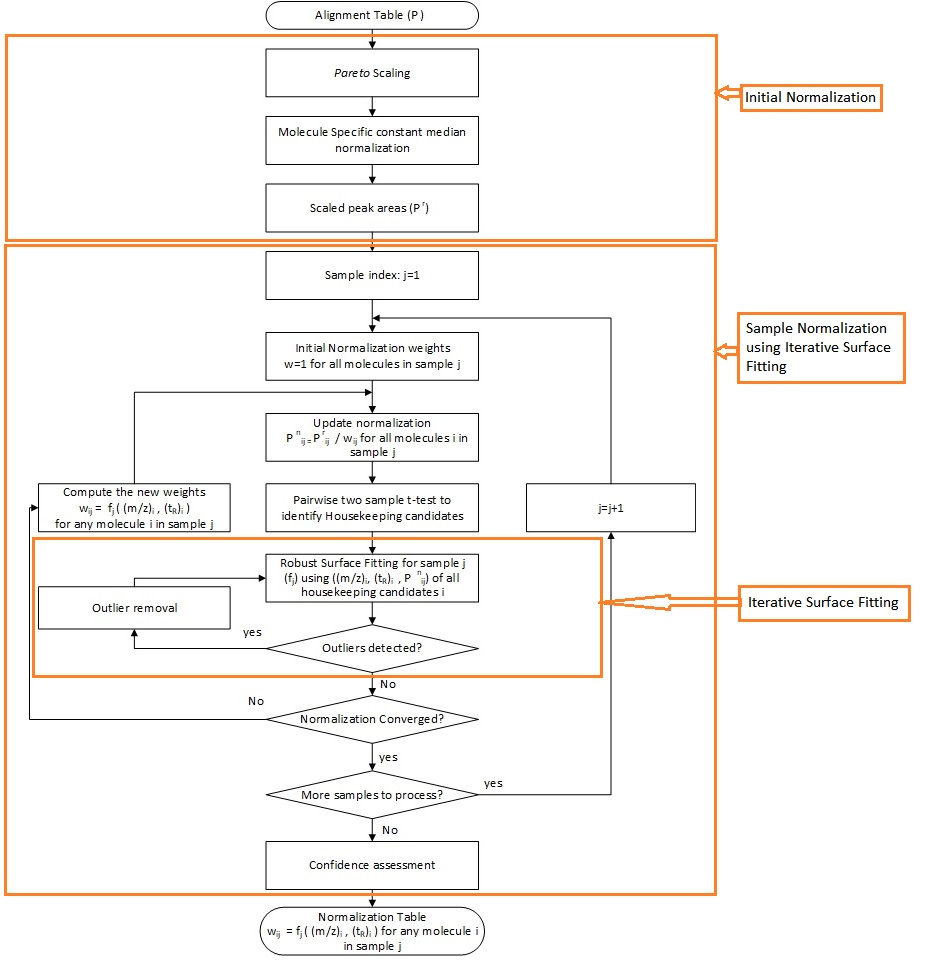
\includegraphics[width=1.1\textwidth]{Work_Flow3}
	\caption{Work flow of the proposed MSN method}
	\label{wf}
\end{figure}

\section{Initial Normalization}
The main aim of this step is to adjust for the differences in fold differences of peak areas between various molecules by converting the data into differences in peak area relative to the scaling factor. \\
\indent First, we apply Pareto Scaling \cite{berg:tar} to each sample across all molecules of the alignment table. Specifically, for each peak area in a selected sample, we apply the transformation:
\begin{eqnarray}\label{eq:0}
P_{ij}'= (P_{ij} - \mu ) / sqrt(s) 
\end{eqnarray}
where $\mu$ is the mean across all molecules of the selected sample and $s$ is the standard deviation of the peak areas of all molecules detected in that sample.\\
\indent After scaling, we proceed to normalize the abundance of each house-keeping molecule by the median of peak areas of that molecule across all samples. First, we compute the median ($Med_i$) of the peak area of a molecule (i) across all samples ($j=1,\dots ,N$). Then, the peak area ratio of each molecule is computed using:
\begin{eqnarray}\label{eq:2}
P_{ij}^r=P_{ij} / Med_i , \text{ $ i=1, \dots ,M$ and $j= 1, \dots ,N.$}
\end{eqnarray}
A table of ratios is then generated for all molecules $P^r$. This table will be used as input to the surface fitting in the next step.  Figure \ref{first_step} shows the selection of house-keeping molecules and median scaling steps.
\begin{figure}
	
	\centering
	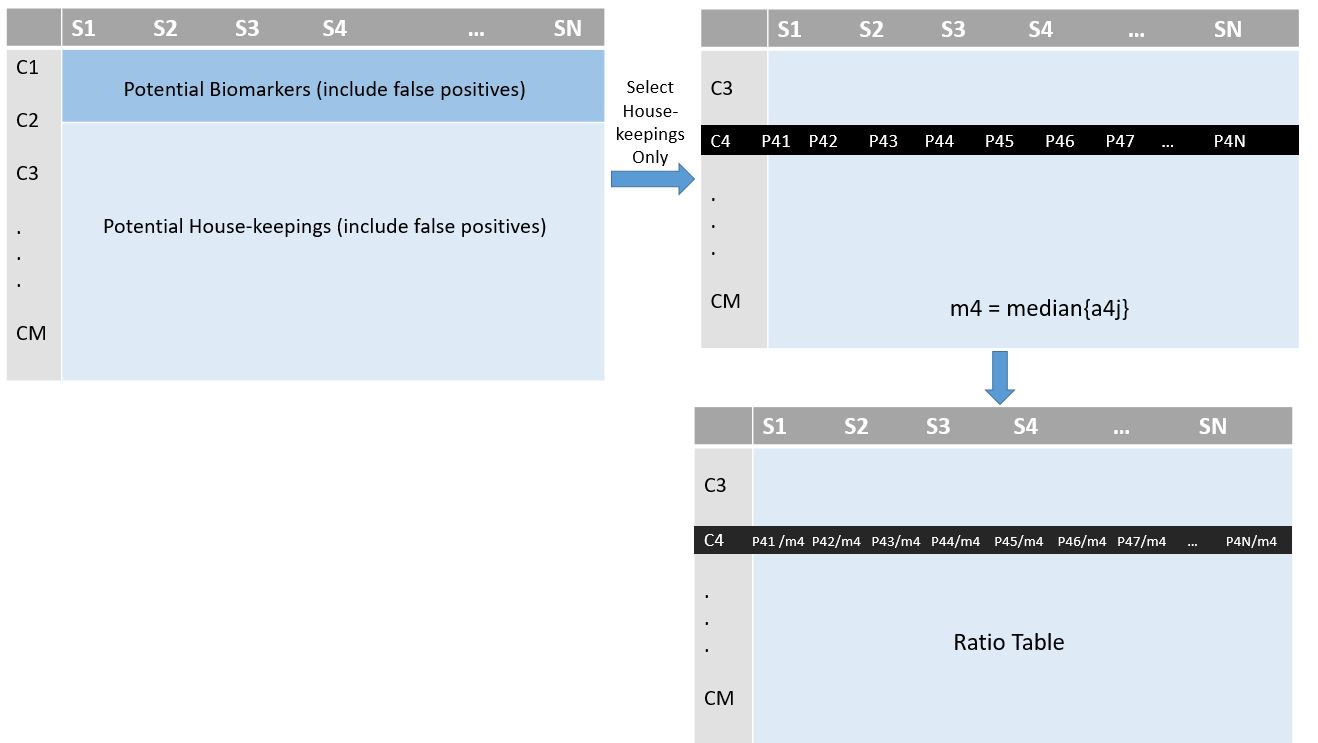
\includegraphics[width=1\textwidth]{first_step}
	\caption{Example of ratio table extraction}
	\label{first_step}
\end{figure}
\section{Sample Normalization Using Iterative Surface Fitting}
The next step of MSN is the main step of our proposed method and consists of sample normalization. The main goal of this step is to estimate weights for normalizing peak areas for all molecules.\\
\indent First, we randomly select one sample and  initialize the weights of all molecules in that sample to unity. These weights will be updated iteratively and the peak areas of the selected sample will be normalized by the updated weights at each iteration.\\
\indent Next, we identify potential house-keepings molecules by applying pairwise
two-tail t-test with sample permutation to deduce the p-value for each molecule. The t statistic for the t-test is computed using:
\begin{eqnarray} 
t={\frac {{\bar {P}}_{1}-{\bar {P}}_{2}}{s_{p}\cdot {\sqrt {{\frac {1}{n_{1}}}+{\frac {1}{n_{2}}}}}}}
\end{eqnarray}
where Sp is the pooled standard deviation
\begin{eqnarray}\label{het} 
 s_{p}={\sqrt {\frac {\left(n_{1}-1\right)s_{P_{1}}^{2}+\left(n_{2}-1\right)s_{P_{2}}^{2}}{n_{1}+n_{2}-2}}}.
\end{eqnarray}
\indent In \ref{het}, $s_{P_1}^2$ and $s_{P_2}^2$ are the unbiased estimators of the variances of the two samples. 
We select the house-keeping molecules as the set of molecules with p-value larger than $ \geq 0.05$. Note that the biomarkers are usually selected by setting $p <0.05$. In the following, we let $H$ denote the set of selected house-keeping molecules.\\
\indent After selecting the house-keepings, we proceed with the surface fitting step. This step will be detailed in section 3.3. \\
\indent After surface fitting, the normalization factor $w_{ij}$ of any molecule $i$ (including those that were not selected as the house-keeping candidates) in the j-th sample can be calculated from the j-th fitted surface function using its (m/z,$t_R$ ) values. The normalized peak area of this molecule is then calculated as:

\begin{eqnarray}\label{eq:3}
P_{ij}^f= P_{ij}^r / w_{ij}
\end{eqnarray}
Using the learned normalization factor $P_{ij}^f$ for the ith molecule in the jth sample, a pairwise t-test is reapplied to all molecules to identify an updated set of house-keeping molecules.
The fitting process for each sample will be repeated until the identified set of house-keepings do not change from iteration to iteration.

\begin{figure}
	
	\centering
	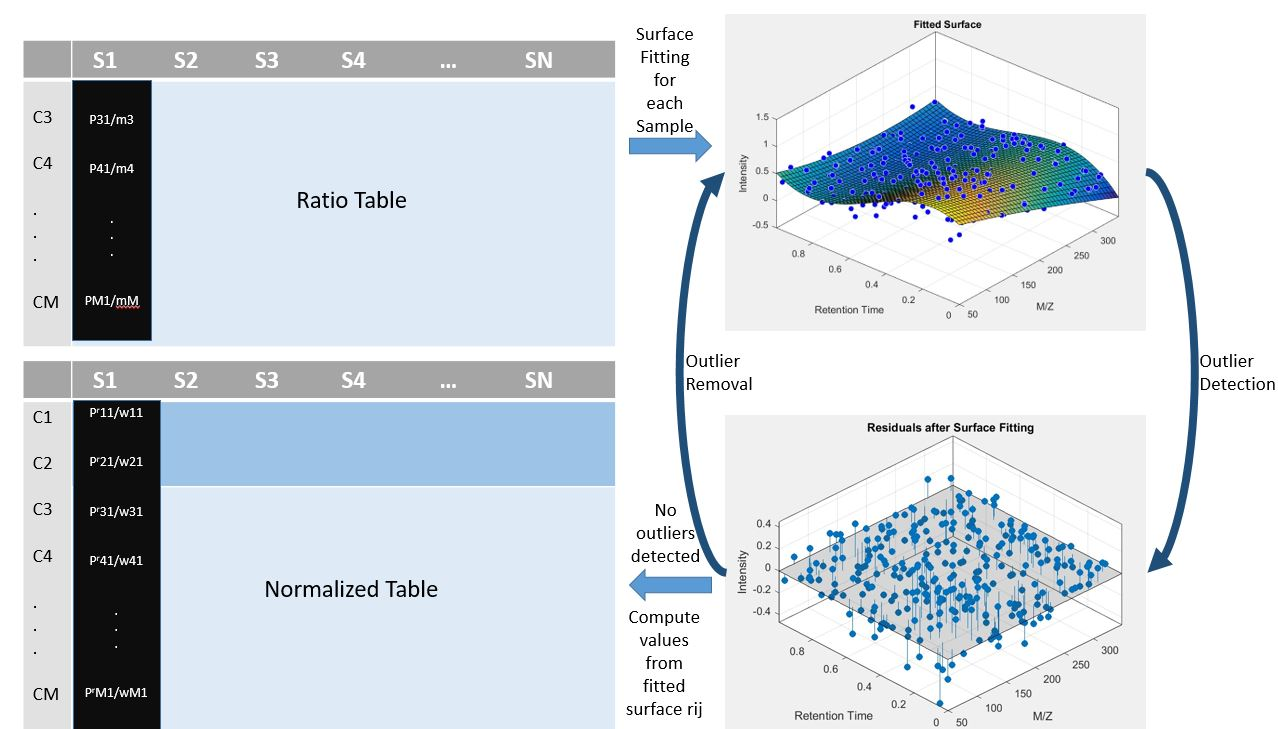
\includegraphics[width=1.1\textwidth]{second_step}
	\caption{Illustration of the iterative process of learning normalization weights and data normalization}
	\label{second_step}
\end{figure}

In Figure \ref{second_step}, we illustrate the iterative surface fitting and outlier detection and removal steps to learn the final normalization weights. 


\section{Robust Surface Fitting}

The main goal of this procedure is to estimate weights for normalizing peak areas for all molecules. To achieve this goal, we treat each sample separately and fit a surface to each one. For sample $j$, the two independent variables ($X$ , $Y$) to the surface fitting function include the m/z value and retention time, $t_R$, of each house-keeping molecule $h_i$. The dependent variable ($Z$) is the peak area ratio, $P^r_{ij}$. This component consists of two iterative steps. The first one fits the surface $ Z= f(X,Y)$. Initially, all house-keeping molecules are used for fitting. We use a Lowess local linear regression function for this step. The optimal fitting function is determined by using the Least Absolute Residual Robust method (LAR). The second iterative step consists of identifying molecules with large residual errors, i.e. outliers. These outliers are typically due to large variations introduced to the peak area of a molecule by random errors or technical variations. For instance, a chromatographic peak may be split into two peaks owing to its poor peak shape during spectrum deconvolution. This will result in a significantly reduced peak area for the low abundance molecules and therefore, a small peak area ratio and large variation in the residue after surface fitting. We use Box-plot for outlier detection since it does not assume residues to have a normal distribution.

The peak area ratios of the identified house-keeping outliers will be removed temporarily for the current fitting task and the remaining house-keeping molecules are used for the next iteration of surface fitting. This iterative process is repeated until no more house-keeping molecules can be detected as outliers. 

\chapter{OUTLIER DETECTION BASED ON FISHER CRITERION}
\indent The Fisher ratio \cite{fld} is used to measure the similarity of two objects on the basis of sets of measurements for each object and a statistical model. For the case of supervised learning, the class for a new object (whose real class is unknown) can be estimated by minimizing, across classes, an average of the Fisher kernel distance from the new object to each known member of the given class. In this thesis, we propose adapting the Fisher criterion to detect outliers.\\
\indent First, we assume the training data belongs to two classes, and in each class $i$ we have $n_i$ samples $P_{n,i}, n=1,\dots , n_i$. The mean of each class is computed using:
\begin{eqnarray}
{\mathbf  {m}}_{i}={\frac  {1}{n_{i}}}\sum _{{n=1}}^{{n_{i}}}{\mathbf  {P}}_{n,i},
\end{eqnarray}
The Fisher Ratio is defined as:
\begin{eqnarray}\label{ratio}
J={\frac  {{\mathbf  {S}}_{B}}{{\mathbf  {S}}_{W}}},
\end{eqnarray}
where $S_B$ is the between class scatter matrix:
\begin{eqnarray}
{\mathbf  {S}}_{B}&=({\mathbf  {m}}_{2}-{\mathbf  {m}}_{1})({\mathbf  {m}}_{2}-{\mathbf  {m}}_{1})^{{{\text{T}}}}
\end{eqnarray}
and $S_W$ is the within class scatter matrix:
\begin{eqnarray}
{\mathbf  {S}}_{W}&=\sum _{{i=1,2}}\sum _{{n=1}}^{{l_{i}}}({\mathbf  {P}}_{n,i}-{\mathbf  {m}}_{i})({\mathbf  {P}}_{n,i}-{\mathbf  {m}}_{i})^{{{\text{T}}}}
\end{eqnarray}


The proposed approach focuses on the similarity among the samples (the replicas) of each class. If there are no outliers, the scatter matrix and thus the ratio will be ideally constant even if we delete one sample from either classes since the information contained in one sample is replicated in all the replicas. On the contrary, if one sample is an outlier, the ratio before deleting this sample will be very different from the ratio after deleting the sample. \\
\indent To illustrate this idea, suppose we have one feature $F1$ in two classes $C1$ and $C2$ where $F_1^{C1}=[f_{c1}^1,f_{c1}^2 \ldots f_{c1}^{n1} ]$ are the samples of feature $F1$ in $C1$, and $F_1^{C2}=[f_{c2}^1,f_{c2}^2 \ldots f_{c2}^{n2} ]$ are the samples of feature $F1$ in $C2$. First, we use equation (\ref{ratio}) to compute the fisher ratio each time  one sample from $C2$ is deleted . This will result in $n_2$ ratios $R=[J_1, J_2 ... J_{n2}]$ where $J_k$ is the fisher ratio after deleting the $k^{th}$ sample $f_{c2}^k$. \\

Ideally, if there are no outliers in class $C2$, all ratios within $R$ should be equal. However, in practice, the samples are not identical, and the ratios should form a distribution. The idea is to identify samples that result in Fisher ratios that do not fit the distribution and label them as outliers. In fact, if one sample (or more) is an outlier then after deleting it, the ratio will change remarkably from the distribution formed by the other ratios. Since we cannot assume that ratios within $R$ fit a known distribution, we use the Boxplot method (chapter 2) to detect the outliers.\\
Figure ~\ref{fish} illustrates our approach to detect outliers based on Fisher Criterion. The Figure includes three examples of detected outliers in compounds with noise added to their samples in class $C2$. The first example is a compound with no outliers detected after applying our algorithm. The second example is when one outlier was detected using our algorithm and the third is when two outliers were detected.\\
\indent The plots on the left of the Figure are the data points of one compound in the two classes $C1$ and $C2$ with noise added to class $C2$.
The plots on the right are the distributions formed by the ratios for different features. The ratios are calculated each time after retrieving one data sample. The red points circled in orange are the points that were selected as outliers from the distribution using Boxplot. The y axis is the ratio value.\\
\indent  One main advantage of our proposed method is that it is applicable to any data with unknown distribution. The absence of  normal distribution or any specific distribution assumption gives it a favor compared to other methods such as Grubbs, GESD and Kimber in terms of applicability. Compared to boxplot, which is a method that is also independent from any distribution assumption, we will show that our method is better in terms of efficiency and classification improvement.
\begin{figure}[t!]
	\centering
	\begin{subfigure}{1\textwidth}
		\centering
		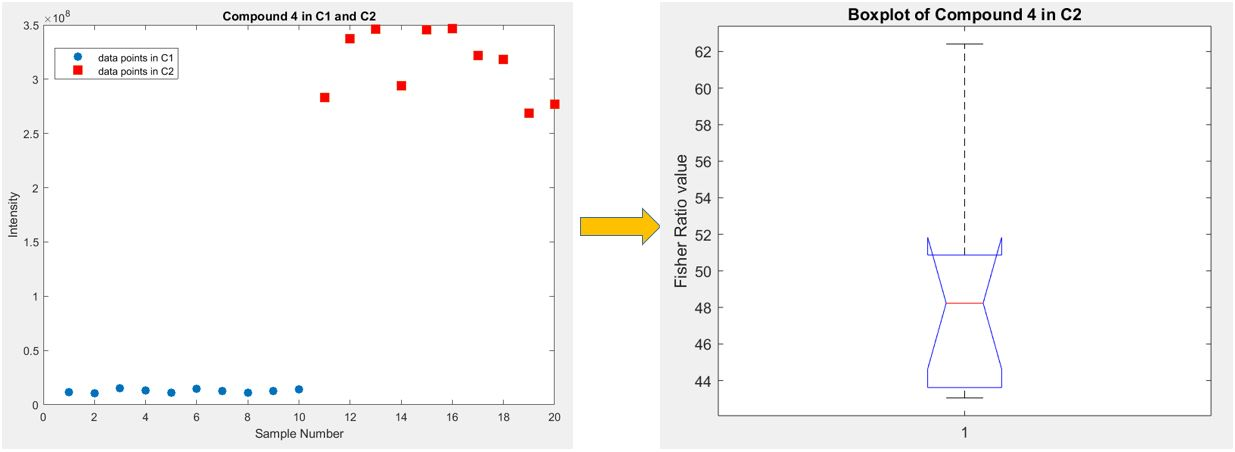
\includegraphics[height=2.1in]{no_outlier}
		\caption{Example 1 with no outlier detected in $C2$}
		\label{fisher1}
	\end{subfigure}%
	 \\
	\begin{subfigure}{1\textwidth}
		\centering
		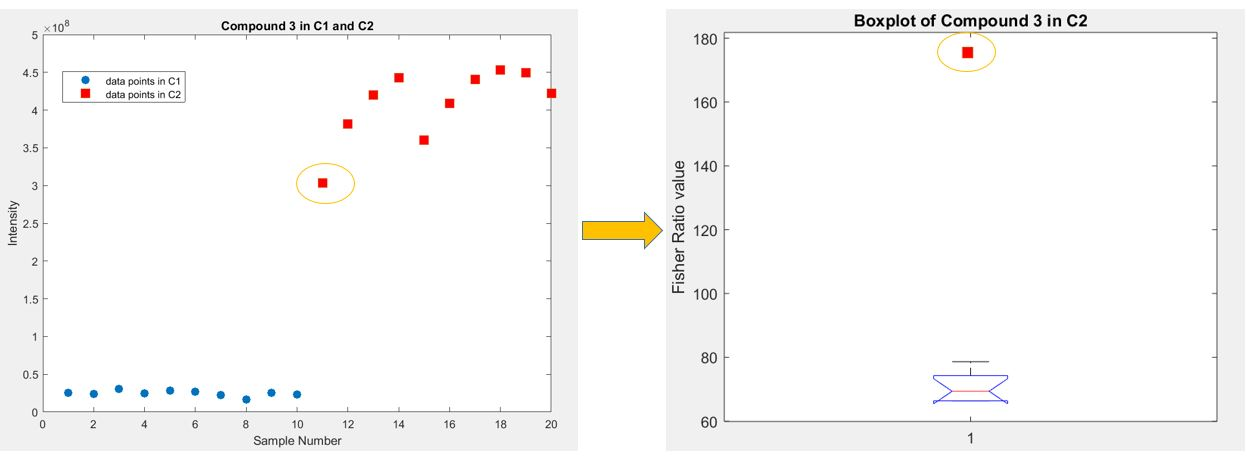
\includegraphics[height=2.1in]{one_outlier}
		\caption{Example 2 with one outlier detected in $C2$}
		\label{fisher2}
	\end{subfigure}

	\begin{subfigure}{1\textwidth}
		\centering
		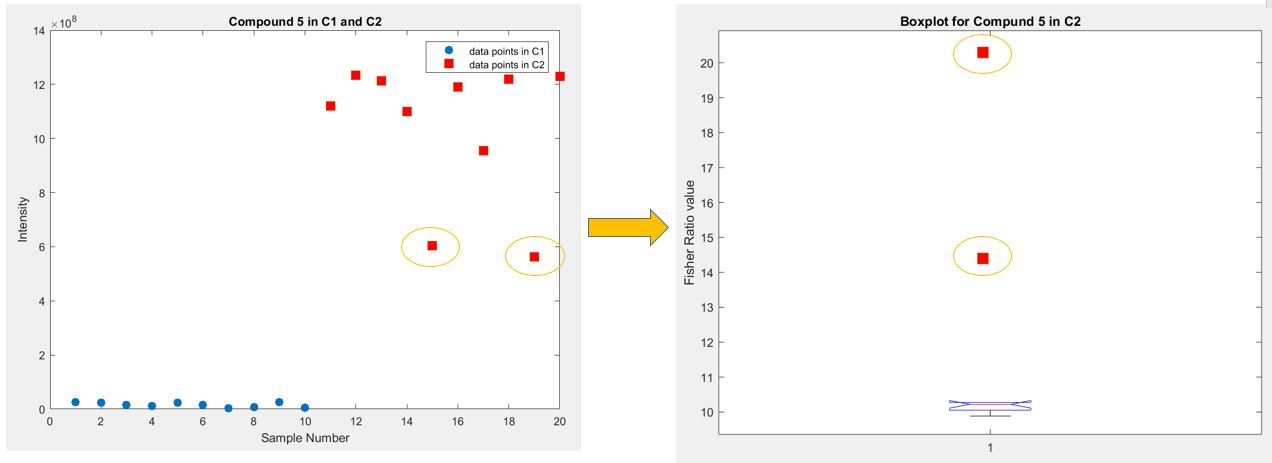
\includegraphics[height=2.1in]{two_outlier}
		\caption{Example 3 with two outlier detected in $C2$}
		\label{fisher3}
	\end{subfigure}
	\caption{Examples of detected outliers in compounds with noise added to their samples in class $C2$}
	\label{fish}
\end{figure}

%\include{3_proposedWork/CDSUcov}
%\include{3_proposedWork/GCMMU}
\chapter{EXPERIMENTAL RESULTS}
The experiments were run on a DELL computer equipped with a 3.6 GHz Intel Xeon processor and a 24 GB RAM.
\section{Example Data Sets}
In these experiments, we used two LC-MS data sets with spiked molecular standards. The first was a metabolomics LC-MS data of mouse liver extract. The second was a proteomics LC-MS data of human urine \cite{christin}.
\begin{itemize}
	\item{ \textbf{Metabolomics data of mouse liver metabolite extract with spiked metabolite standards}}
\end{itemize}


This data was generated in our lab by extracting metabolites from a pooled mouse liver sample using a solvent mixture water:methabol $(v:v = 8:2)$. The metabolite extract was then equally split into 60 aliquots to form 6 sample groups $(G0, G1,\ldots,G5 )$ with (n=10 in each group). Different volumes of a mixture of 48 metabolite standards were spiked in each sample. The concentrations of each metabolite standard spiked in the 6 sample groups were $0 \mu M$, $0.625 \mu M$, $1.25 \mu M$, $2.5 \mu M$, $5 \mu M$  and $10 \mu M$, respectively. All samples were analyzed on a Q Exactive HF Hybrid Quadrupole-Orbitrap Mass Spectrometer equipped with a C18 RP column and a HILIC column configured in parallel. The MS was operated in both positive and negative modes to acquire the full MS and MS/MS spectra for each metabolite. LC-MS data were first analyzed using MetSign software \cite{metsign} for spectrum deconvolution, metabolite assignment and cross-sample peak list alignment.\\

\begin{itemize}
\item{\textbf{Proteomics data of human urine with spiked peptide mixtures} }
\end{itemize}

This publicly available data set was generated from 8 different sample groups with 5 samples in each
group. The data set was introduced in (\cite{christin}). Briefly, a pooled urine sample, collected from 15 healthy females and 35 healthy males over the age range of 26.9 to 72.9 years, was spiked with a tryptic digest (V5111; Promega, Madison, WI) of bovine carbonic anhydrase (C3934, Uniprot entry: P00921; Sigma, Steinheim, Germany), as well as with seven synthetic peptides at eight different dilutions: 6.25, 12.5, 25, 50, 100, 200, 400, and 2000 times dilution. The final data covers peaks with m/z values from 280 to 1500 amu, with a constant resolution of 0.1 amu, and retention times between 30 and 85 min, resulting in a final common peak list of 29,529 features, with 151 of those originating from the added peptides (i.e. biomarkers).

\section{Validation of the proposed MSN algorithm by data classification}


The LC-MS metabolomics data was used to validate the proposed MSN method and its performance was compared with existing normalization methods outlined in Chapter 2. First, we considered groups $G0$ and $G5$ (the easiest case since $G5$ samples were spiked with the highest concentration of each metabolite standard) and normalized the data using the different methods. Next, for each normalized data, we used PLS-DA as a classifier to assign a confidence value showing the likelihood of each metabolite to be a biomarker. Then, using these confidence values and the ground truth, we generated an ROC curve and computed the area under the curve (AUC) within $[0 \ldots 0.1]$. Thus, if all biomarkers (i.e. spiked-in metabolite standards) could be detected with no false positives, then $AUC = 0.1$, else $AUC < 0.1$. Next, to analyze the effect of noise on the different normalization methods, we corrupted one of the samples from $G0$ with multiplicative noise. Specifically, for each metabolite $i$, we modified its peak area using $P'_{i,k}=(1+ \epsilon )P_{i,k}$, where $k$ is the sample to be corrupted, $\epsilon$ is a random number uniformly distributed in the range $[0,U]$ with $U=5\%$, $10 \%$, $15 \% $,and $20 \% $ (the case of noise free samples correspond to U=0). Due to the randomness of the added noise, we repeated this experiment 10 times and reported the mean and standard deviations of the AUC. 

\begin{figure}
	
	\centering
	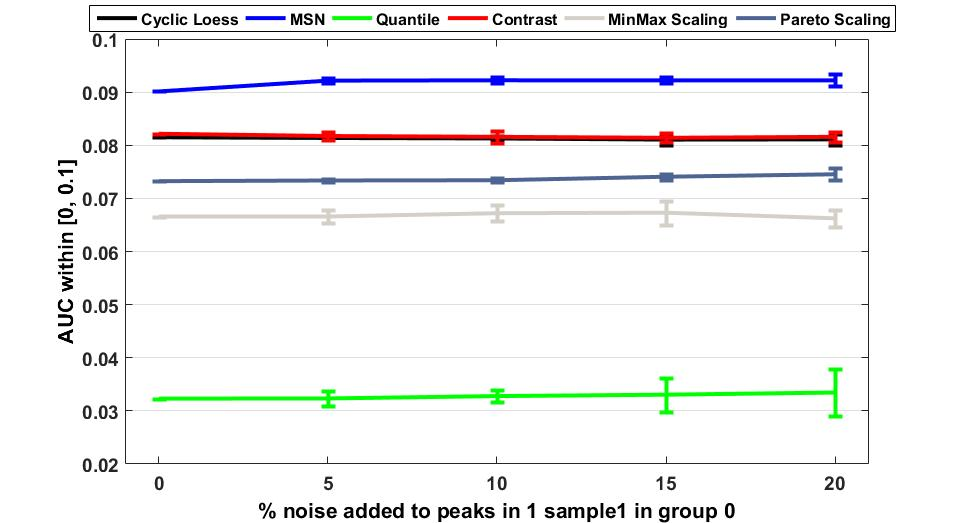
\includegraphics[width=1\textwidth]{ErrorBar_PLSDA_s3}
	\caption{Comparison of the performance of the proposed MSN method to 5 normalization methods when groups G0 and G5 are considered and as we vary the noise level on one sample in G0 in Liver Extraction Data.}
	\label{ErrorBar_PLSDA_s3}
\end{figure}

\begin{figure}
	
	\centering
	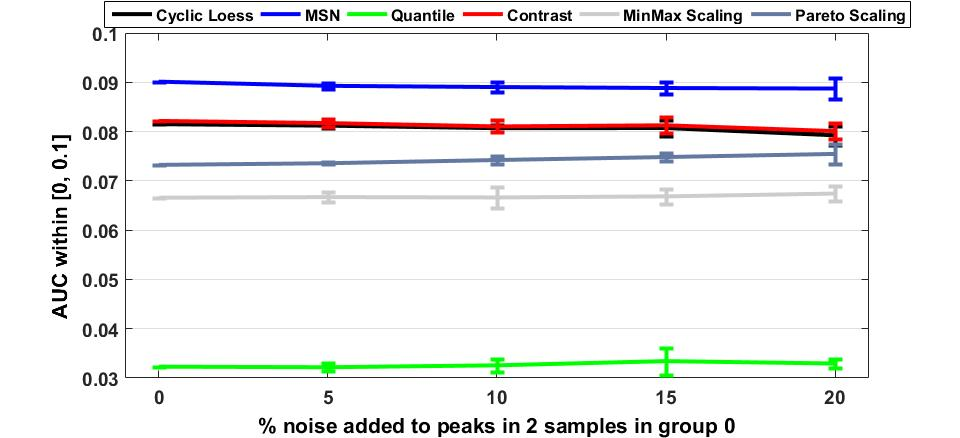
\includegraphics[width=1\textwidth]{ErrorBar_PLSDA_2samples}
	\caption{Comparison of the performance of the proposed MSN method to 5 normalization methods when groups G0 and G5 are considered and as we vary the noise level on two samples in G0 in Liver Extraction Data.}
	\label{ErrorBar_PLSDA_2samples}
\end{figure}

Figure ~\ref{ErrorBar_PLSDA_s3} shows the results obtained by all normalization methods for all 5 levels of added noise. As it can be seen, the proposed MSN normalization is significantly better than all other methods as it has the largest AUC values at all noise levels. Second, the MSN (and most other methods) are robust to noise since the performance does not degrade as noise increases from $0\%$ to $20\%$. Third, we note the small standard deviation indicating the consistency of the results across the multiple runs with different random noise. 

In a second experiment, we added noise to two samples from group $G0$ (i.e. samples 3 and 6) and repeated the same experiment. The results are shown in Figure ~\ref{ErrorBar_PLSDA_2samples} where similar behavior can be concluded. 

We performed multiple other evaluations by adding noise to samples from $G5$ and by considering other groups $G1 \ldots G4$. As expected, the performance degraded as we considered groups containing metabolite standards with less spiked-in concentrations. However, MSN remained as the most robust method and performed significantly better than the other 5 methods. In Figure ~\ref{ErrorBar_PLSDA_2samplesingroup0-3} we show the results when we considered groups G0 and G3 and when two samples from G0 were corrupted by noise. 

\begin{figure}
	
	\centering
	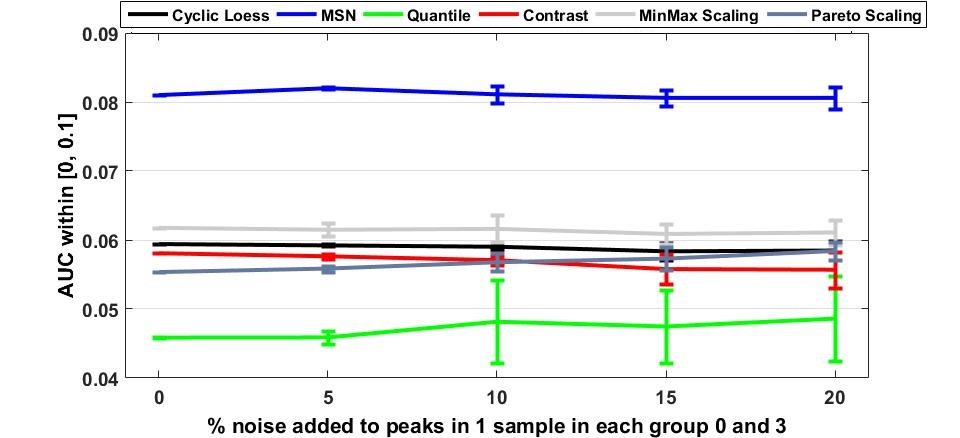
\includegraphics[width=1\textwidth]{ErrorBar_PLSDA_2samplesingroup0-3}
	\caption{Comparison of the performance of the proposed MSN methods to 5 normalization methods when groups G0 and G3 are considered and as we vary the noise level on two samples in G0 in the Liver Extraction Data.}
	\label{ErrorBar_PLSDA_2samplesingroup0-3}
\end{figure}

To analyze the results further, in Figure ~\ref{MZ-data_surfaceOfS3} and ~\ref{RT-data_surfaceOfS3} we display the surface fitted to the potential house-keeping metabolites of sample 3 before and after adding $20\%$ noise. To simplify the visualization of the 3-D surface, Figure ~\ref{MZ-data_surfaceOfS3} displays normalization factor $w_{ij}$ vs. m/z and Figure ~\ref{RT-data_surfaceOfS3} displays $w_{ij}$  vs.  $t_R$. As it can be seen, $w_{ij}$  tends to increase as we add noise. Normalizing by higher values will reduce the effect of noise. 



\begin{figure}
	
	\centering
	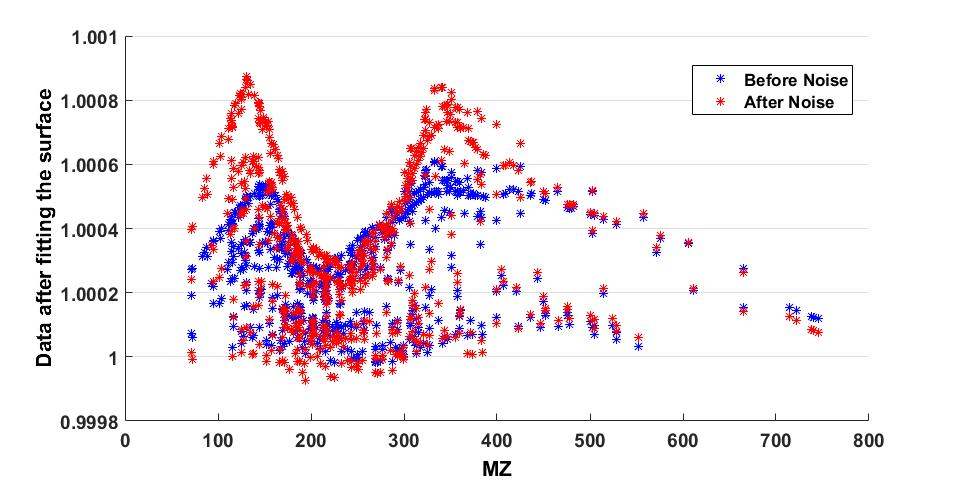
\includegraphics[width=1\textwidth]{MZ-data_surfaceOfS3}
	\caption{Learned normalization factors, as a function of the m/z values, for the potential house-keeping metabolites of sample 3 in $G0$ before and after adding $20\%$ noise in Liver Extraction Data.}
	\label{MZ-data_surfaceOfS3}
\end{figure}

\begin{figure}
	
	\centering
	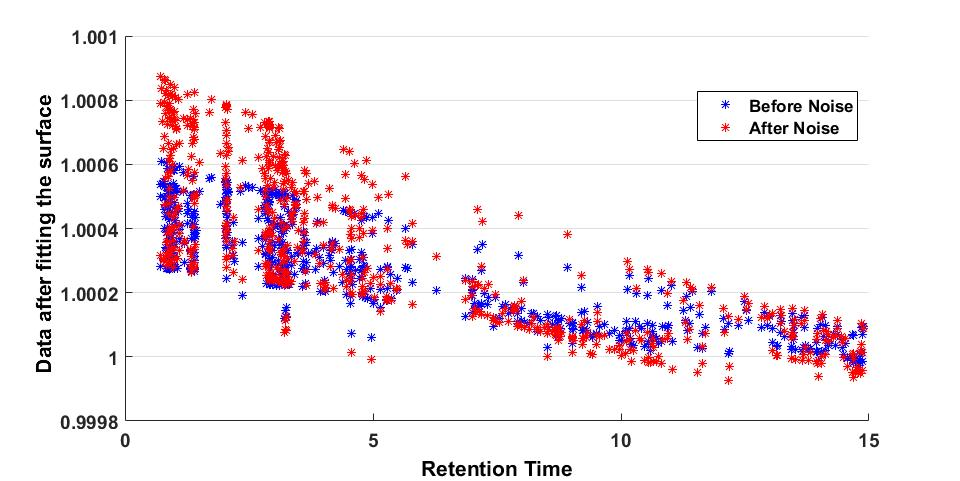
\includegraphics[width=1\textwidth]{RT-data_surfaceOfS3}
	\caption{Learned normalization factors, as a function of the retention time, for the potential house-keeping metabolites of sample 3 in $G0$ before and after adding $20\%$ noise in Liver Extraction Data.}
	\label{RT-data_surfaceOfS3}
\end{figure}



\begin{figure}
	
	\centering
	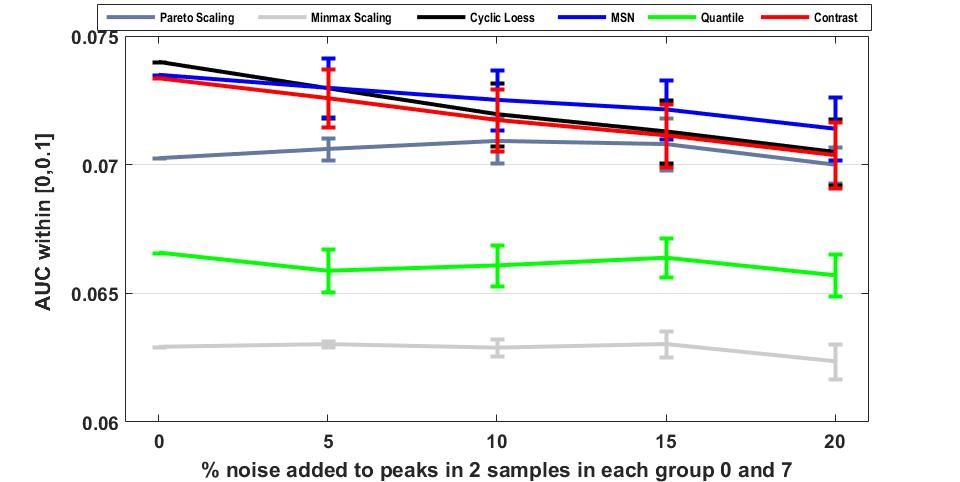
\includegraphics[width=1\textwidth]{g0-7_errorbar}
	\caption{Comparison of the performance of the proposed MSN methods to 5 normalization methods as we vary the noise level and the samples affected by noise in G0 and G7 in the Human Urine Data.}
	\label{g07errorbar}
\end{figure}
\begin{figure}
	
	\centering
	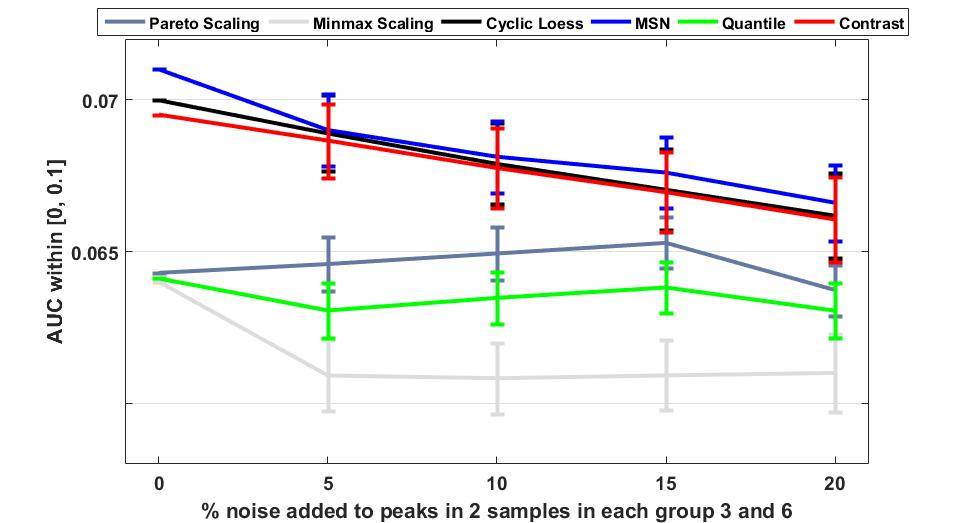
\includegraphics[width=1\textwidth]{g3-6_errobar}
	\caption{Comparison of the performance of the proposed MSN methods to 5 normalization methods as we vary the noise level and the samples affected by noise in G3 and G6 in the Human Urine Data.}
	\label{g36errobar}
\end{figure}
For the second data set, we performed similar experiments as with the metabolomics data set. First, we considered groups $G0$ and $G7$, normalized the data, and used the PLS-DA  to assign a confidence value indicating the likelihood of each feature to be a biomarker. Then, using these confidence values and the ground truth, we computed the area under the curve (AUC) within $[0 \ldots 0.1]$. For this experiment, we corrupted two samples from $G0$ and two samples from $G7$ with multiplicative noise. The corrupted samples were chosen randomly. As with the metabolomics data, we repeated each normalization 10 times and reported the mean and standard deviations of the AUC. The results are shown in Figure ~\ref{g07errorbar}.


As it can be seen, the proposed MSN normalization outperforms other methods as it has the largest AUC values at all noise levels.
In another validation test, we added noise to two samples from group $G0$ and two samples from group $G3$ and repeated the same experiment. The results are shown in Figure ~\ref{g36errobar}, where the same conclusion can be observed.

\section{Evaluation of the proposed Outlier Detection Algorithm}

We used LC-MS metabolomics data to validate the proposed outlier detection method. First, we considered groups $G0$ and $G5$ as it is the easiest case and applied our outlier detection algorithm based on Fisher Criterion. Second, we applied feature selection algorithms to assign a confidence value showing the likelihood of each metabolite to be a biomarker. Using these confidence values and the ground truth, we generated an ROC curve and computed the area under the curve (AUC). Next, we corrupted one or more of the samples from $G0$ and $G5$ by adding outliers to those samples. For a selected samples we added or subtracted a multiple number of sigmas $ k \times \sigma$ with sigmas the standard deviations of each molecule in that group. We will try different values of $k$ and different number of corrupted samples. \\
\indent In TABLE \ref{fld} we report the Area Under the Curve of the classification using the Ensemble Feature Selection method \cite{ali} of $G0$ and $G5$ before and after applying our proposed outlier detection method. 

\begin{table}[h!]
	\centering
	\caption{AUC of Classification Results of $G0$ and $G5$ of Noisy Data after applying our proposed method}
	\begin{tabular}{|c|c|c|c|} 
		\hline
		\textbf{Applied Noise} & \textbf{AUC After ODFC} & \textbf{AUC After OD using Boxplot} &	\textbf{AUC Before OD} \\ [0.5ex] 
		\hline\hline
		\textbf{2 outliers, N= 3$\sigma$
		} & 0.0909 & 0.0840 & 0.0800 \\
		\hline
		\textbf{3 outliers, N= 3$\sigma$
		} & 0.0815 & 0.0775 & 0.0773 \\
		\hline
		\textbf{4 outliers, N= 3$\sigma$} & 0.0741 & 0.0647 & 0.0647\ \\
		
		\hline
		\textbf{3 outliers, N= 4$\sigma$} & 0.0814 & 0.0677 & 0.0681\\
		\hline
		\textbf{4 outliers, N= 4$\sigma$} & 0.0563 & 0.0360 & 0.0353 \\ 
		\hline
	\end{tabular}
	\label{fld}
\end{table}


\begin{table}[h!]
	\centering
	\caption{AUC of Classification Results of $G0$ and $G3$ of Noisy Data after applying our proposed method}
	\begin{tabular}{|c|c|c|c|} 
		\hline
		\textbf{Applied Noise} & \textbf{AUC After ODFC} & \textbf{AUC After OD using Boxplot} &	\textbf{AUC Before OD} \\ [0.5ex] 
		\hline\hline
		\textbf{2 outliers, N= 3$\sigma$
		} & 0.0708  & 0.0674 & 0.0662\\
		\hline
		\textbf{3 outliers, N= 3$\sigma$
		} & 0.0545 & 0.0518 & 0.0491 \\
		\hline
		\textbf{4 outliers, N= 3$\sigma$} & 0.0411  & 0.0392 & 0.0378 \\
		
		\hline
		\textbf{3 outliers, N= 4$\sigma$} & 0.0545  & 0.0518 & 0.0491\\
		\hline
		\textbf{4 outliers, N= 4$\sigma$} & 0.0547 & 0.0368 & 0.0366	 \\ 
		\hline
	\end{tabular}
	\label{fld2}
\end{table}


As it can be seen, after applying the proposed outlier detection method, the AUC has increased in all the experiments. Since the classification accuracy is very high (perfect classification will result in AUC=0.1), the improvement is not very significant. Thus, we can conclude that, the removal of the outliers using the proposed method has improved the performance of the classification.\\
\indent We performed a second experiment, similar to the first one, except that we used groups $G0$ and $G3$ and we measure the AUC of the classification using the Ensembe Feature Selection algortihm \cite{ali}.The results are reported in TABLE \ref{fld2} where a similar conclusion can be observed. In fact, for this harder case, there is more room for improvements and our outlier detection algorithm improved the classification more than the previous experiment.


\chapter{CONCLUSIONS AND POTENTIAL FUTURE WORK}

\section{Discussion}

By performing multiple experiments using both proteomics and metabolomics data sets, we showed that the proposed MSN approach consistently outperforms many of the commonly used normalization methods for the considered applications. We should note here that similar to our MSN, both Cyclic Loess and Contrast based methods are based on Loess Local regression. However, MSN has two main advantages. First, instead of fitting one global surface to all samples, MSN uses a local approach and adapts the surface fitting to each sample. Second, it integrates normalization, house-keeping detection, and robust surface fitting in an iterative process. Third, it invlolves the outlier detection method to reduce the effect of potential technical variation on normalization and biomarker discovery. Thus, it can recover from an initial bad scaling or inaccurate set of house-keeping molecules. 

The proposed MSN approach assumes that the abundance levels of a certain number of molecules do not change between samples and controls (i.e. house-keeping molecules). In general, this requirement can be easily met in most proteomics and metabolomics studies. However, in extreme cases, the proposed MSN may not work if the entire proteome or metabolome is changed. In this case, any numerical normalization method will fail. The only alternative is to use internal standards, tissue weight, or cell numbers, depending on the experiment design. Another potential challenge is that the house-keeping molecules may have extremely skewed distribution in the retention time - m/z plane. In this case, the normalization factors will have large variation for the molecules located in sparse regions.



\section{Conclusions}

A new approach for normalizing proteomics and metabolomics data, entitled molecule specific normalization (MSN), was developed. MSN first identifies a group of molecules whose abundance levels were not affected by the biological treatment (i.e. house-keeping molecules). Then, it adopts a robust surface fitting strategy to minimize the molecular profile difference of the house-keeping molecules across samples. The normalization factor of each molecular peak is determined by its retention time and m/z within each sample. Using a metabolomics data set and a proteomics data set, we applied different degrees of noise on random samples and compared the performance of MSN to five other normalization methods. We showed that MSN is more robust to noise than any of the five other methods. This is due to the fact that MSN is based on a robust surface fitting approach and also treats the noise that is applied to each sample separately. We also showed that MSN has improved the classification performance by around 24\% on average of the different experiments with the metabolomics data and by around 5\% on average with the proteomics data. \\
\indent A new approach for outlier detection was also introduced. This approach is based on the Fisher Criterion to detect data points that do not belong to the data distribution. A remarkable change in the criterion after removing one data point at a time indicates that the removed data point is an outlier.\\
The performance of the classification has slightly ameliorated with 2\% improvement for classification using the two groups $G0$ and $G5$ and with 5\% improvement for classification using the two groups $G0$ and $G3$.





%\bibliographystyle{h-physrev}
\begin{spacing}{0.9}
\bibliographystyle{LatexClass/IEEEbib}
%\renewcommand{\bibname}{References} % changes the header; default: Bibliography
\bibliography{backmatter/proposalBib} % adjust this to fit your BibTex file
\end{spacing}
\singlespace

\chapter*{\normalfont{CURRICULUM VITAE}}
\addcontentsline{toc}{part}{\normalfont{CURRICULUM VITAE}}%\addtotoc{Curriculum Vitae}
\begin{tabbing}
{\bf NAME:} \hspace{5em} \= Ameni Trabelsi\\\\
{\bf ADDRESS:}  \> Computer Engineering \& Computer Science Department\\
\> Speed School of Engineering \\
\> University of Louisville \\
\> Louisville, KY 40292
\end{tabbing}
\subsection*{EDUCATION:}
\begin{description}
\item \hspace{8.5em}\begin{tabular}{l}M.S., Computer Science \& Engineering \\
May 2018\\
\textbf{University of Louisville}, \emph{Louisville, Kentucky}\end{tabular}
\item \hspace{8.5em}\begin{tabular}{l}B.Eng., Computer Science Engineering\\
June 2016\\
\textbf{Tunisia Polytechnic School},
\emph{Tunis, Tunisia}\end{tabular}
\end{description}

\subsection*{AWARDS AND CERTIFICATIONS:}
\begin{enumerate}
	 \item CECS Master of Science Award, May 2018.
 	\item Certification of Seeds For the Future Program Training (HUAWEI CHINA), September 2015.
\end{enumerate}
\subsection*{PROJECTS:}
\begin{enumerate}
	\item Molecule Specific Normalization: Robust Normalization Algorithm for Omics Data using Surface Fitting
	\item Outlier Detection Method Using Fisher Criterion: A New Approach for Outlier Detection for Omics Data using Fisher Criterion
	\item Image Annotation using Partially Labeled Data: An Image Annotation Approach using Multiple Instance Learning to Label Partially Labeled Data
	
\end{enumerate}
\cleardoublepage


\end{document}
